%%%%%%%%%%%%%%%%%%%%%%%%%%%%%%%%%%%%%%%%%%%%%%%%%%%%%%%%%%%%%%%%%%%%%%%%%%%
%                                                                         %
%                     ENERGY DEPOSITION SIMULATIONS                       %
%                                                                         %
%%%%%%%%%%%%%%%%%%%%%%%%%%%%%%%%%%%%%%%%%%%%%%%%%%%%%%%%%%%%%%%%%%%%%%%%%%%

The average energy deposited by a neutron and gamma reaction was investigated for different film thickness to determine if an optimal thickness does exits in a geometry similar to \autoref{fig:EDepSimGeo}.
\autoref{fig:SimEDep} shows that the energy deposition of the gamma quickly falls off as the films get thinner, while it isn't until the neutron films become on the order of the range of the triton that the energy deposition is impacted.
\autoref{fig:EDepPosSim} examines the impact of where the interaction took place in the film on the energy deposition.
The geometry for this simulation is once again \autoref{fig:EDepSimGeo}, where the beam spot is \SI{3}{\mm} and the area of the detector face is \SI{10}{\cm}. 
The interaction position is then defined to be distance to the first interaction of the beam in the material along the direction of the beam.
It is observed that for neutrons events that take place within the center of the films tend to deposit a large majority of their energy in the film, while events that occur on the edge of the film have partial energy depositions in accordance with the ranges of the charged particles.
A Compton spectra is observed in the photon energy deposition. 
A secondary effect in having a backing material is also observed for photons in which there is a heightened energy deposition for interactions that occur in the film but near the boundary and electrons are back scattered into the detector material.
\begin{figure}
  \centering
  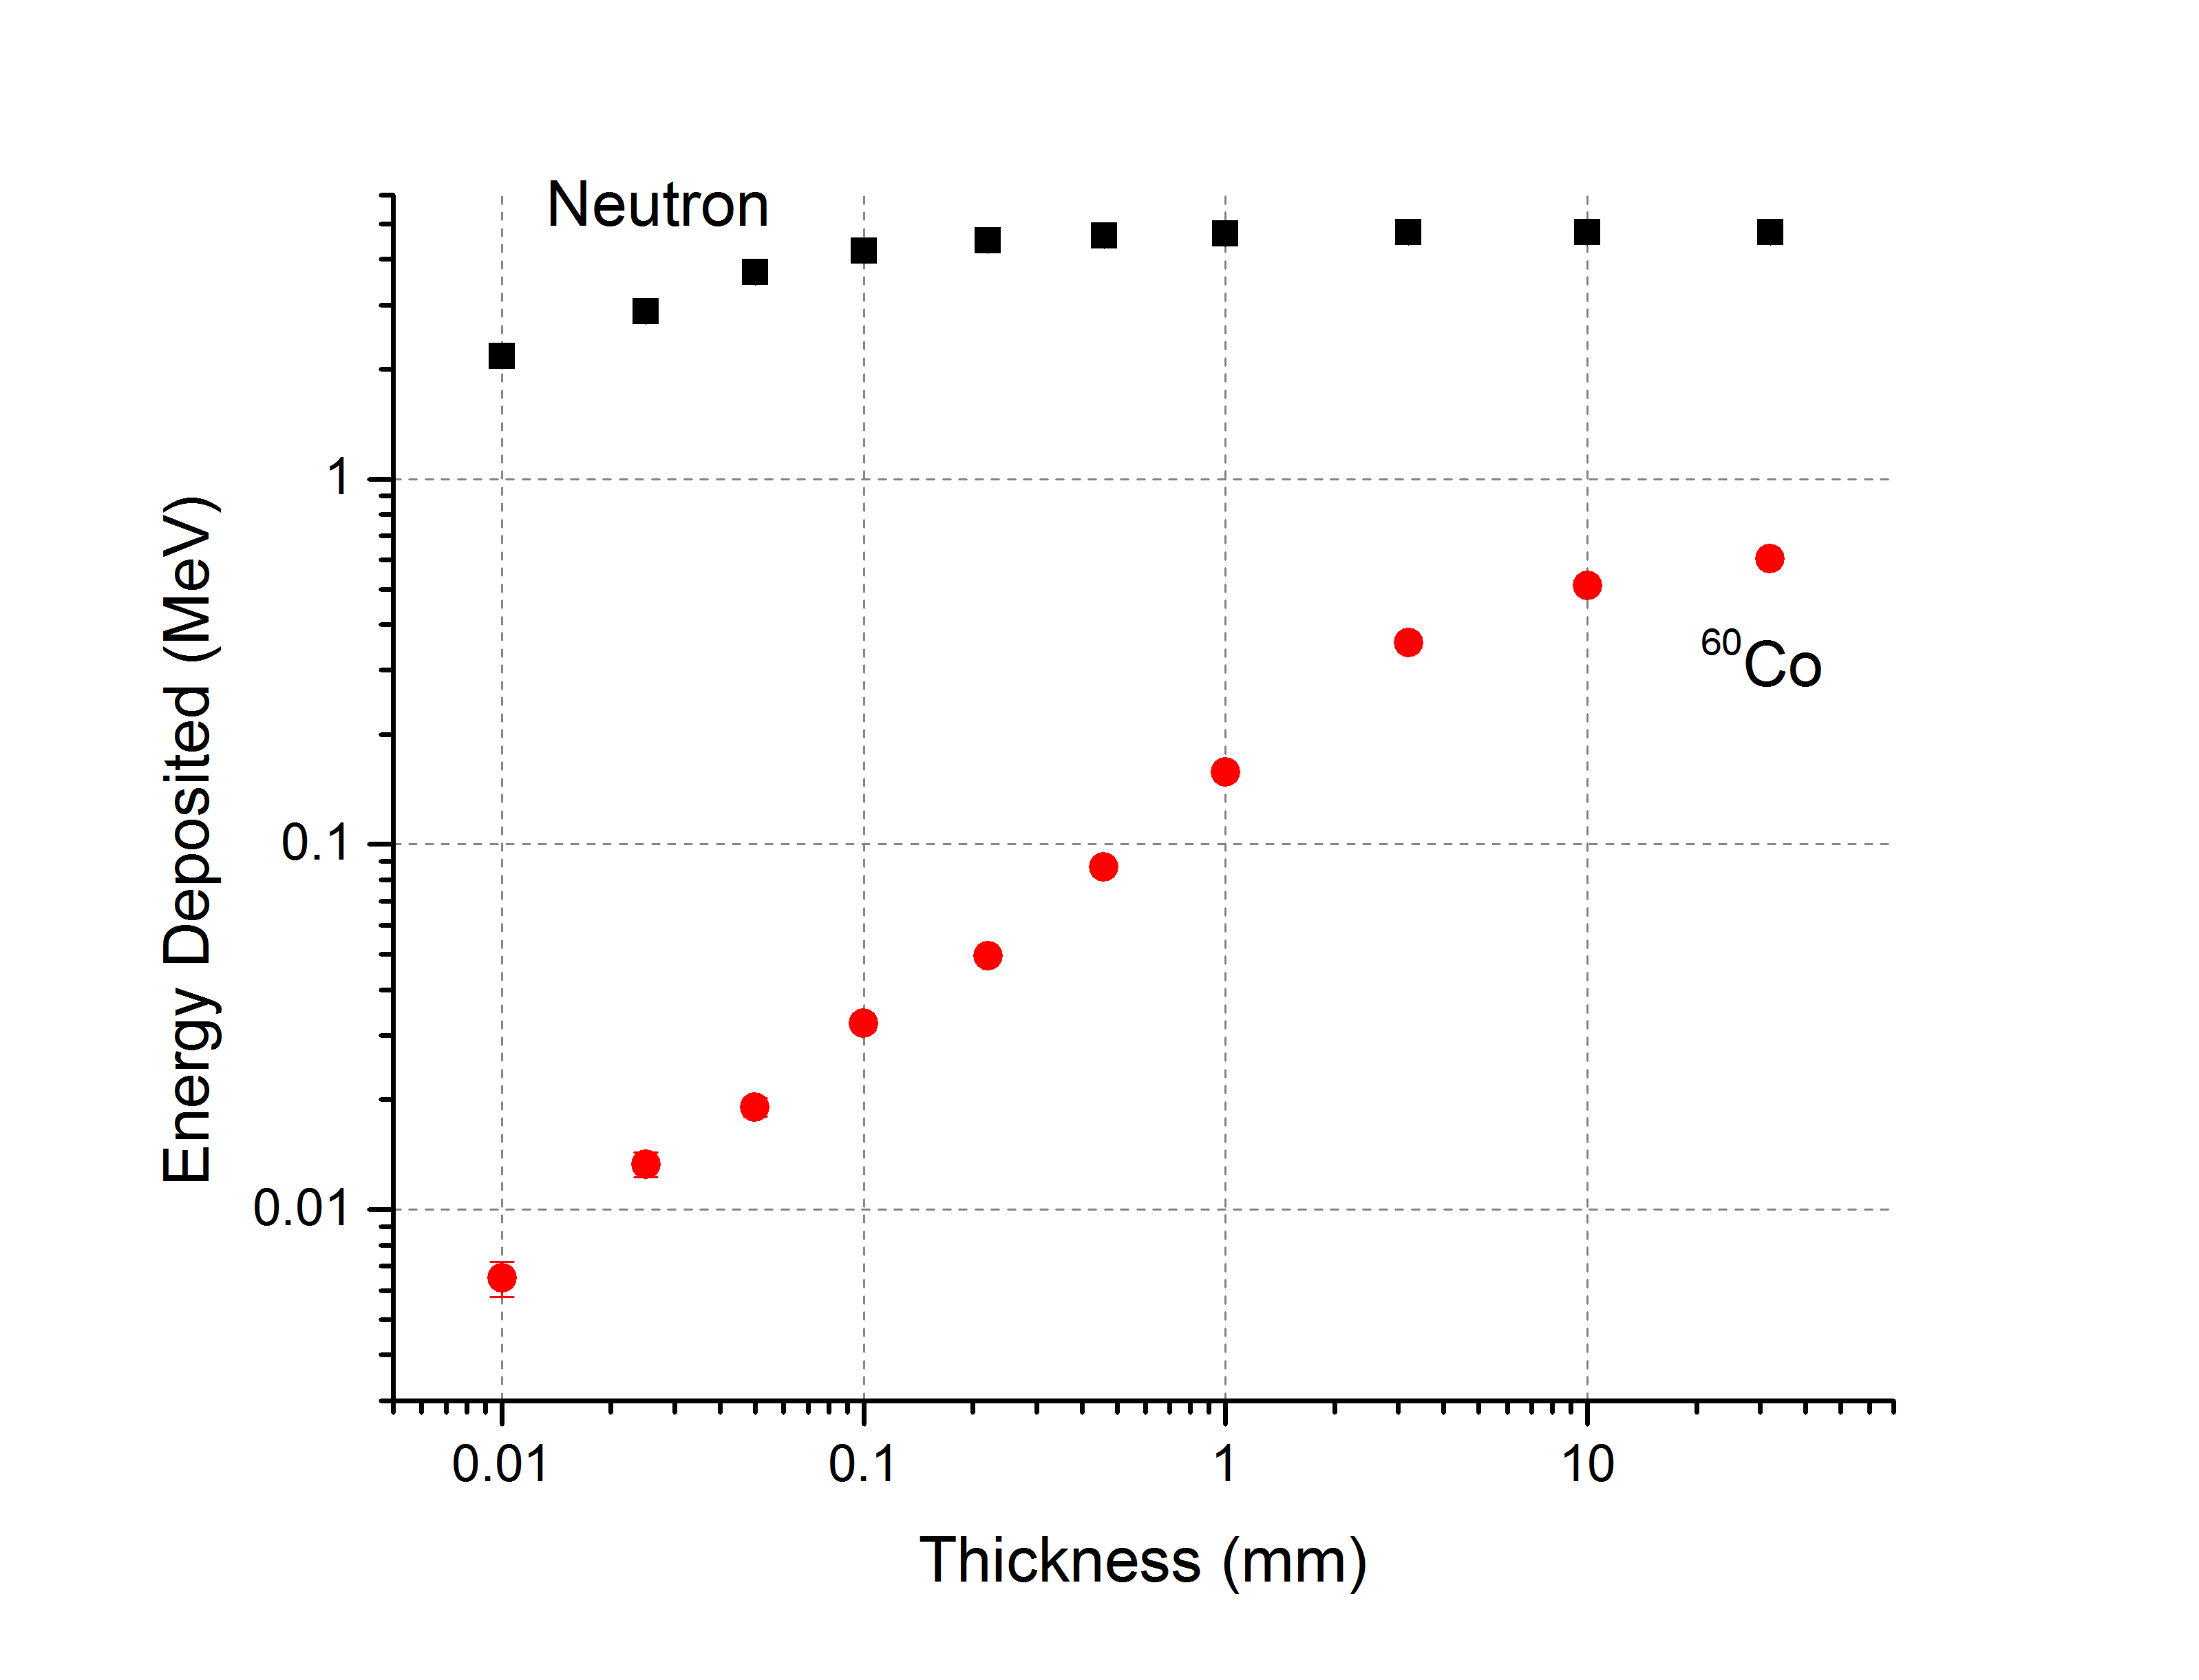
\includegraphics[width=0.6\textwidth]{SimulatedEnergyDeposition}
  \caption[Simulated Energy Deposition and Film Thickness]{Simulated energy deposition and film thickness.  As the films get much thinner it is very unlikely for gamma events to deposition all of their energy, while above \SI{50}{\um} there is very little impact on the energy deposited by neutrons.}
  \label{fig:SimEDep}
\end{figure}

\begin{figure*}[ht]
	\centering
	\begin{subfigure}[b]{0.45\textwidth}
    		\includegraphics[width=\textwidth]{{posEDepCo600.025}.png}
		\caption{ \SI{25}{\um} Gamma (\iso[60]{Co})}
	\end{subfigure}%
	~
	\begin{subfigure}[b]{0.45\textwidth}
    		\includegraphics[width=\textwidth]{{posEDepCo6010.0}.png}
		  \caption{ \SI{1}{\cm} Gamma (\iso[60]{Co})}
	\end{subfigure}%
	
  \begin{subfigure}[b]{0.45\textwidth}
    		\includegraphics[width=\textwidth]{{posEDepneutron0.025}.png}
		\caption{ \SI{25}{\um} Neutron}
	\end{subfigure}%
	~
	\begin{subfigure}[b]{0.45\textwidth}
    		\includegraphics[width=\textwidth]{{posEDepneutron10.0}.png}
		  \caption{ \SI{1}{\cm} Neutron}
	\end{subfigure}%
	\caption[Simulated Energy Deposition and Position]{Simulated average energy depositions and the position of the first interactions. The beam is considered to be incident on position 0, and thus interactions that occur on the front of the film have a much higher probability depositing all of their energy. Events that occur on the edge of the film much less likely to deposit all of their available energy.}
	\label{fig:EDepPosSim}
\end{figure*}

\autoref{fig:simKinE} illustrates the simulated kinetic energy of secondary electrons from Compton scattering and from alpha and triton interactions.
It is observed that kinetic energy of the secondary electrons from the neutron reaction products have predominately energies in the kilo-volt range, while the Compton scattering electrons have energies in hundreds of kilo-volts range. 
However, it should be noted that there is only one secondary electron from a Compton scattering and multiple secondary electrons from the reaction products.
\autoref{fig:ReacProdDist} shows the distribution of the number of secondary electrons from the alpha and triton and their kinetic energy.
\begin{figure}[ht]
    \centering
    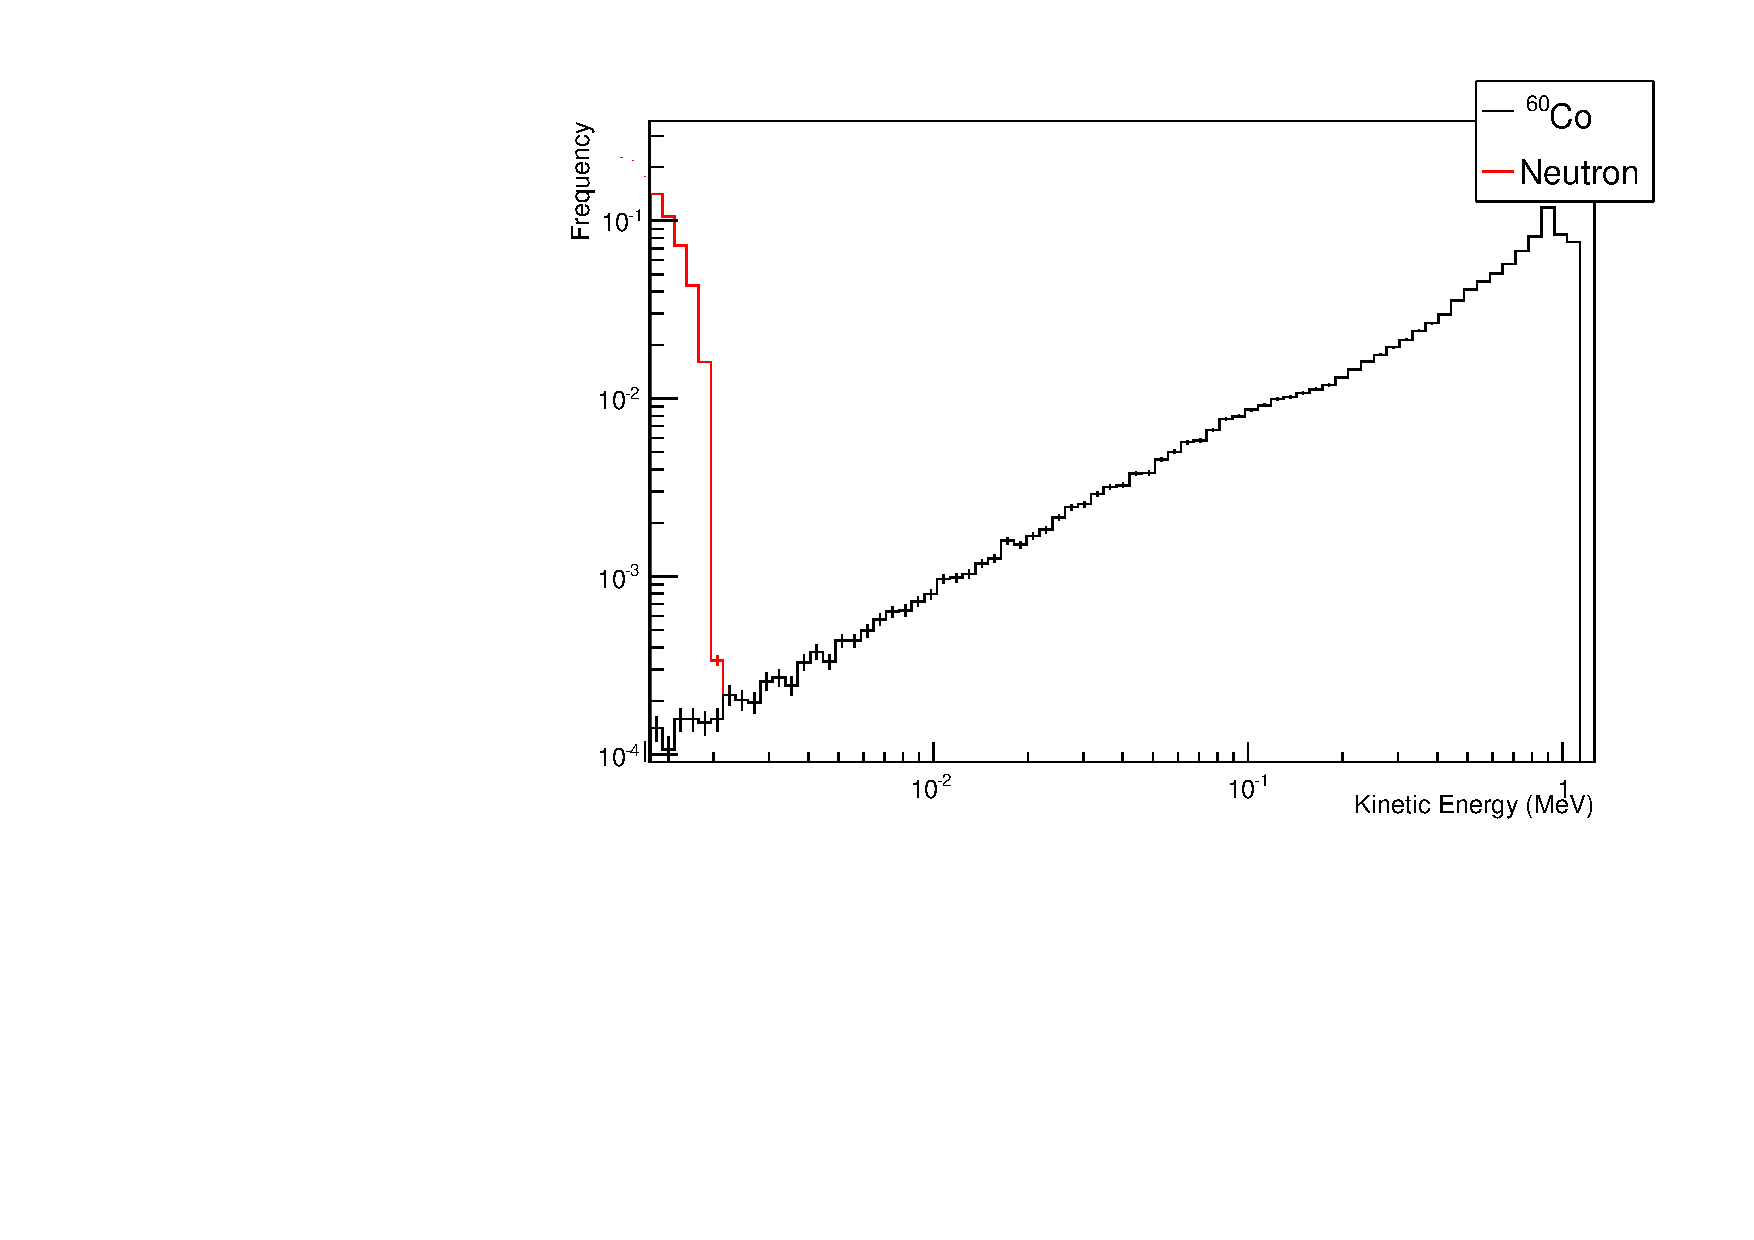
\includegraphics[width=\textwidth]{NGSecElecKinEDist}
    \caption{Simulated Kinetic Energy of Secondary Electrons from Compton Scattering and from \iso[6]{Li} reaction products}
    \label{fig:simKinE}
\end{figure}
\begin{figure*}[ht]
	\centering
	\begin{subfigure}[b]{0.45\textwidth}
    		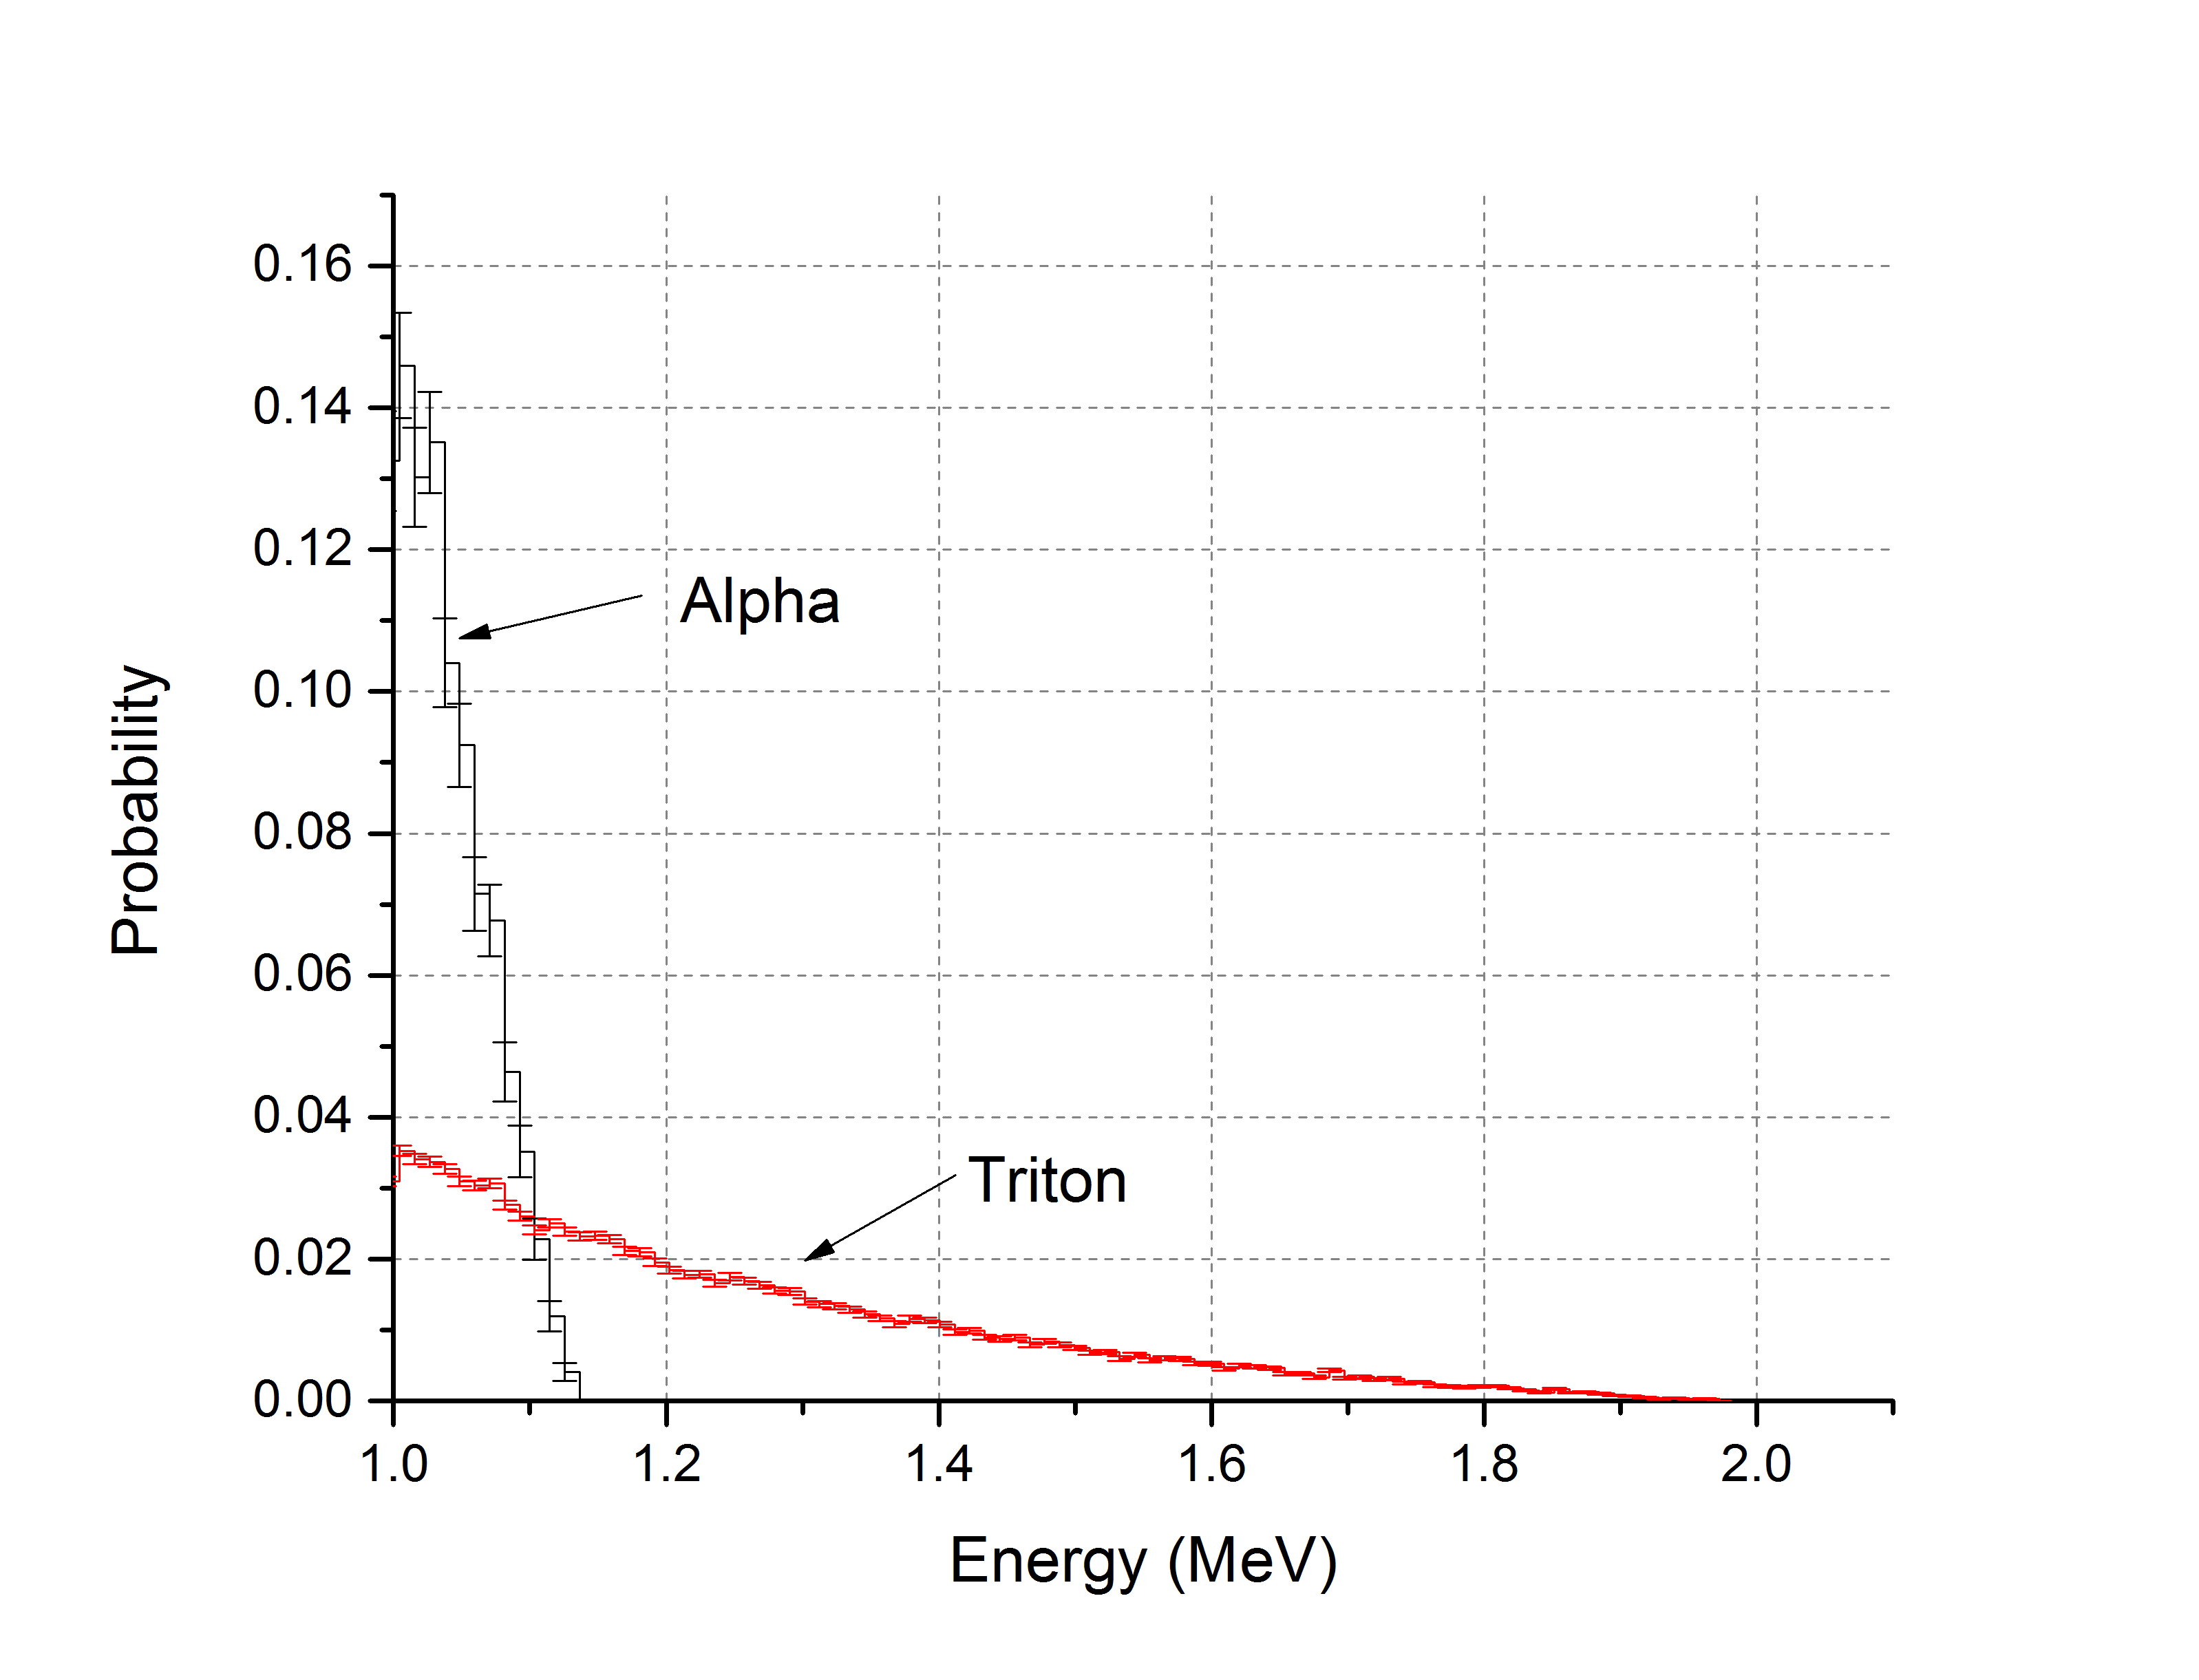
\includegraphics[width=\textwidth]{AlphaTritonSecElecKinEDist}
		\caption{Alpha and Triton Secondary Electron Kinetic Energy Distribution}
	\end{subfigure}%
	~
	\begin{subfigure}[b]{0.45\textwidth}
    		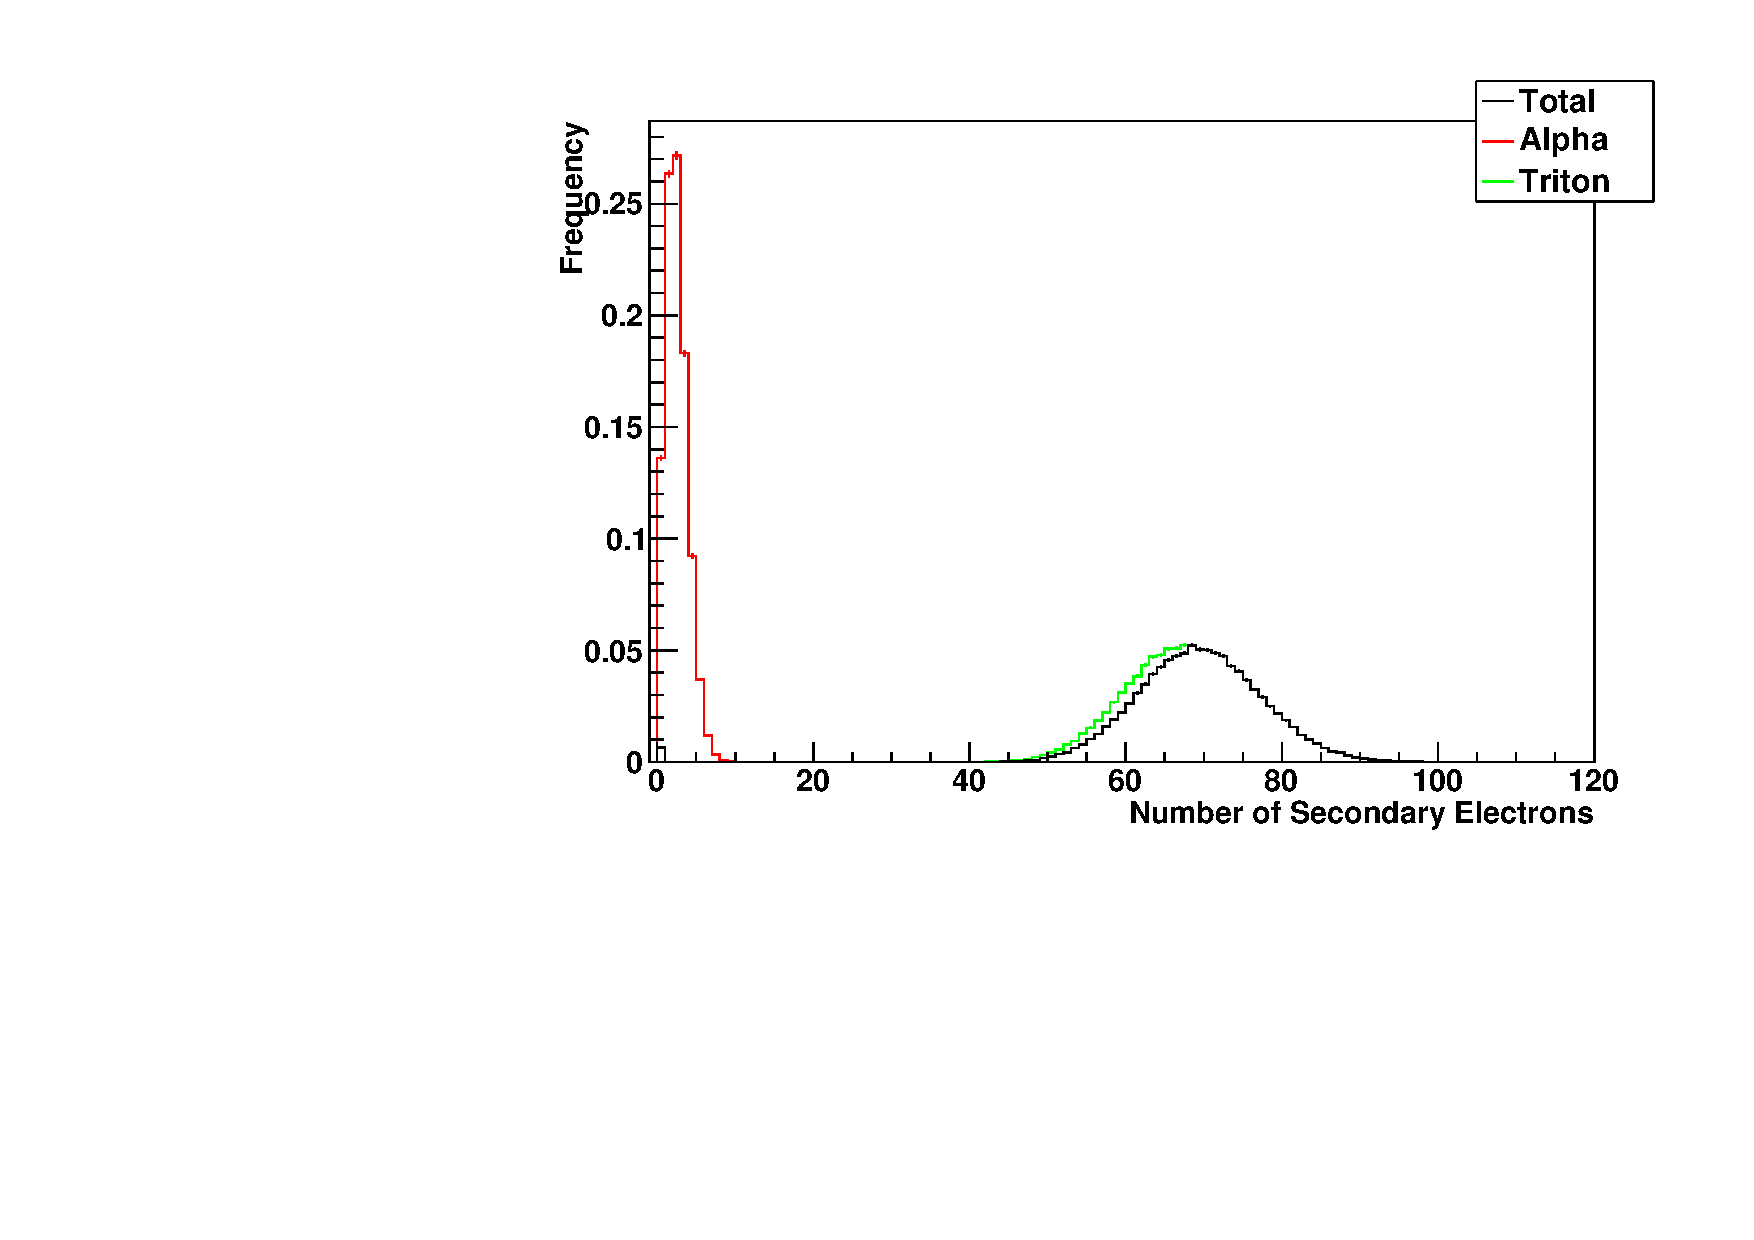
\includegraphics[width=\textwidth]{NeutronNumSecElec}
		\caption{Number of Secondary Electrons Produced Per Neutron Interaction}
	\end{subfigure}%
	\caption{Neutron Reaction Products Secondary Electrons Energies}
	\label{fig:ReacProdDist}
\end{figure*}

The average energy deposited was computed for each thickness and normalized by the incident energy for gammas by the Q-value of the reaction for neutrons, and is presented in Table ~\ref{tab:FractionEDep}.
For thickness greater than \SI{150}{\um} there is little benefit in increasing the thickness of the film in terms of energy deposition by neutrons, since over 90\% of the energy is being deposited in the film.
\begin{table}[ht]
    \caption{Fractional Energy Deposition for Various Thickness}
	\centering
	\begin{tabular}{c | c c}
	Thickness & Gamma Fraction & Neutron Fraction \\
	\hline
	\hline
	\SI{15}{\um} & 0.010 & 0.531 \\
	\SI{25}{\um} & 0.013 & 0.634 \\
	\SI{50}{\um} & 0.017 & 0.782 \\
	\SI{150}{\um} & 0.032 & 0.927 \\
	\SI{300}{\um} & 0.052 & 0.964 \\
	\SI{600}{\um} & 0.087 & 0.982 \\
	\SI{1}{\mm} & 0.130 & 0.989 \\
	\SI{1}{\cm} & 0.425 & 0.998 \\
	\end{tabular}
  \label{tab:FractionEDep}
\end{table}

%%%%%%%%%%%%%%%%%%%%%%%%%%%%%%%%%%%%%%%%%%%%%%%%%%%%%%%%%%%%%%%%%%%%%%%%%%%
%                                                                         %
%                  Light Yield and Energy Deposition                      %
%                                                                         %
%%%%%%%%%%%%%%%%%%%%%%%%%%%%%%%%%%%%%%%%%%%%%%%%%%%%%%%%%%%%%%%%%%%%%%%%%%%
\section{Light Yield and Energy Deposition}
The energy deposition and light yield were also investigated by simulations in the GEANT4 environment for polystyrene based films (light output 1,000 photons per MeV).
These simulations (summarized in \autoref{fig:EDepLightYield}) show that as expected the light output was linear with the energy deposition.
\begin{figure*}[ht]
	\centering
	\begin{subfigure}[b]{0.45\textwidth}
    		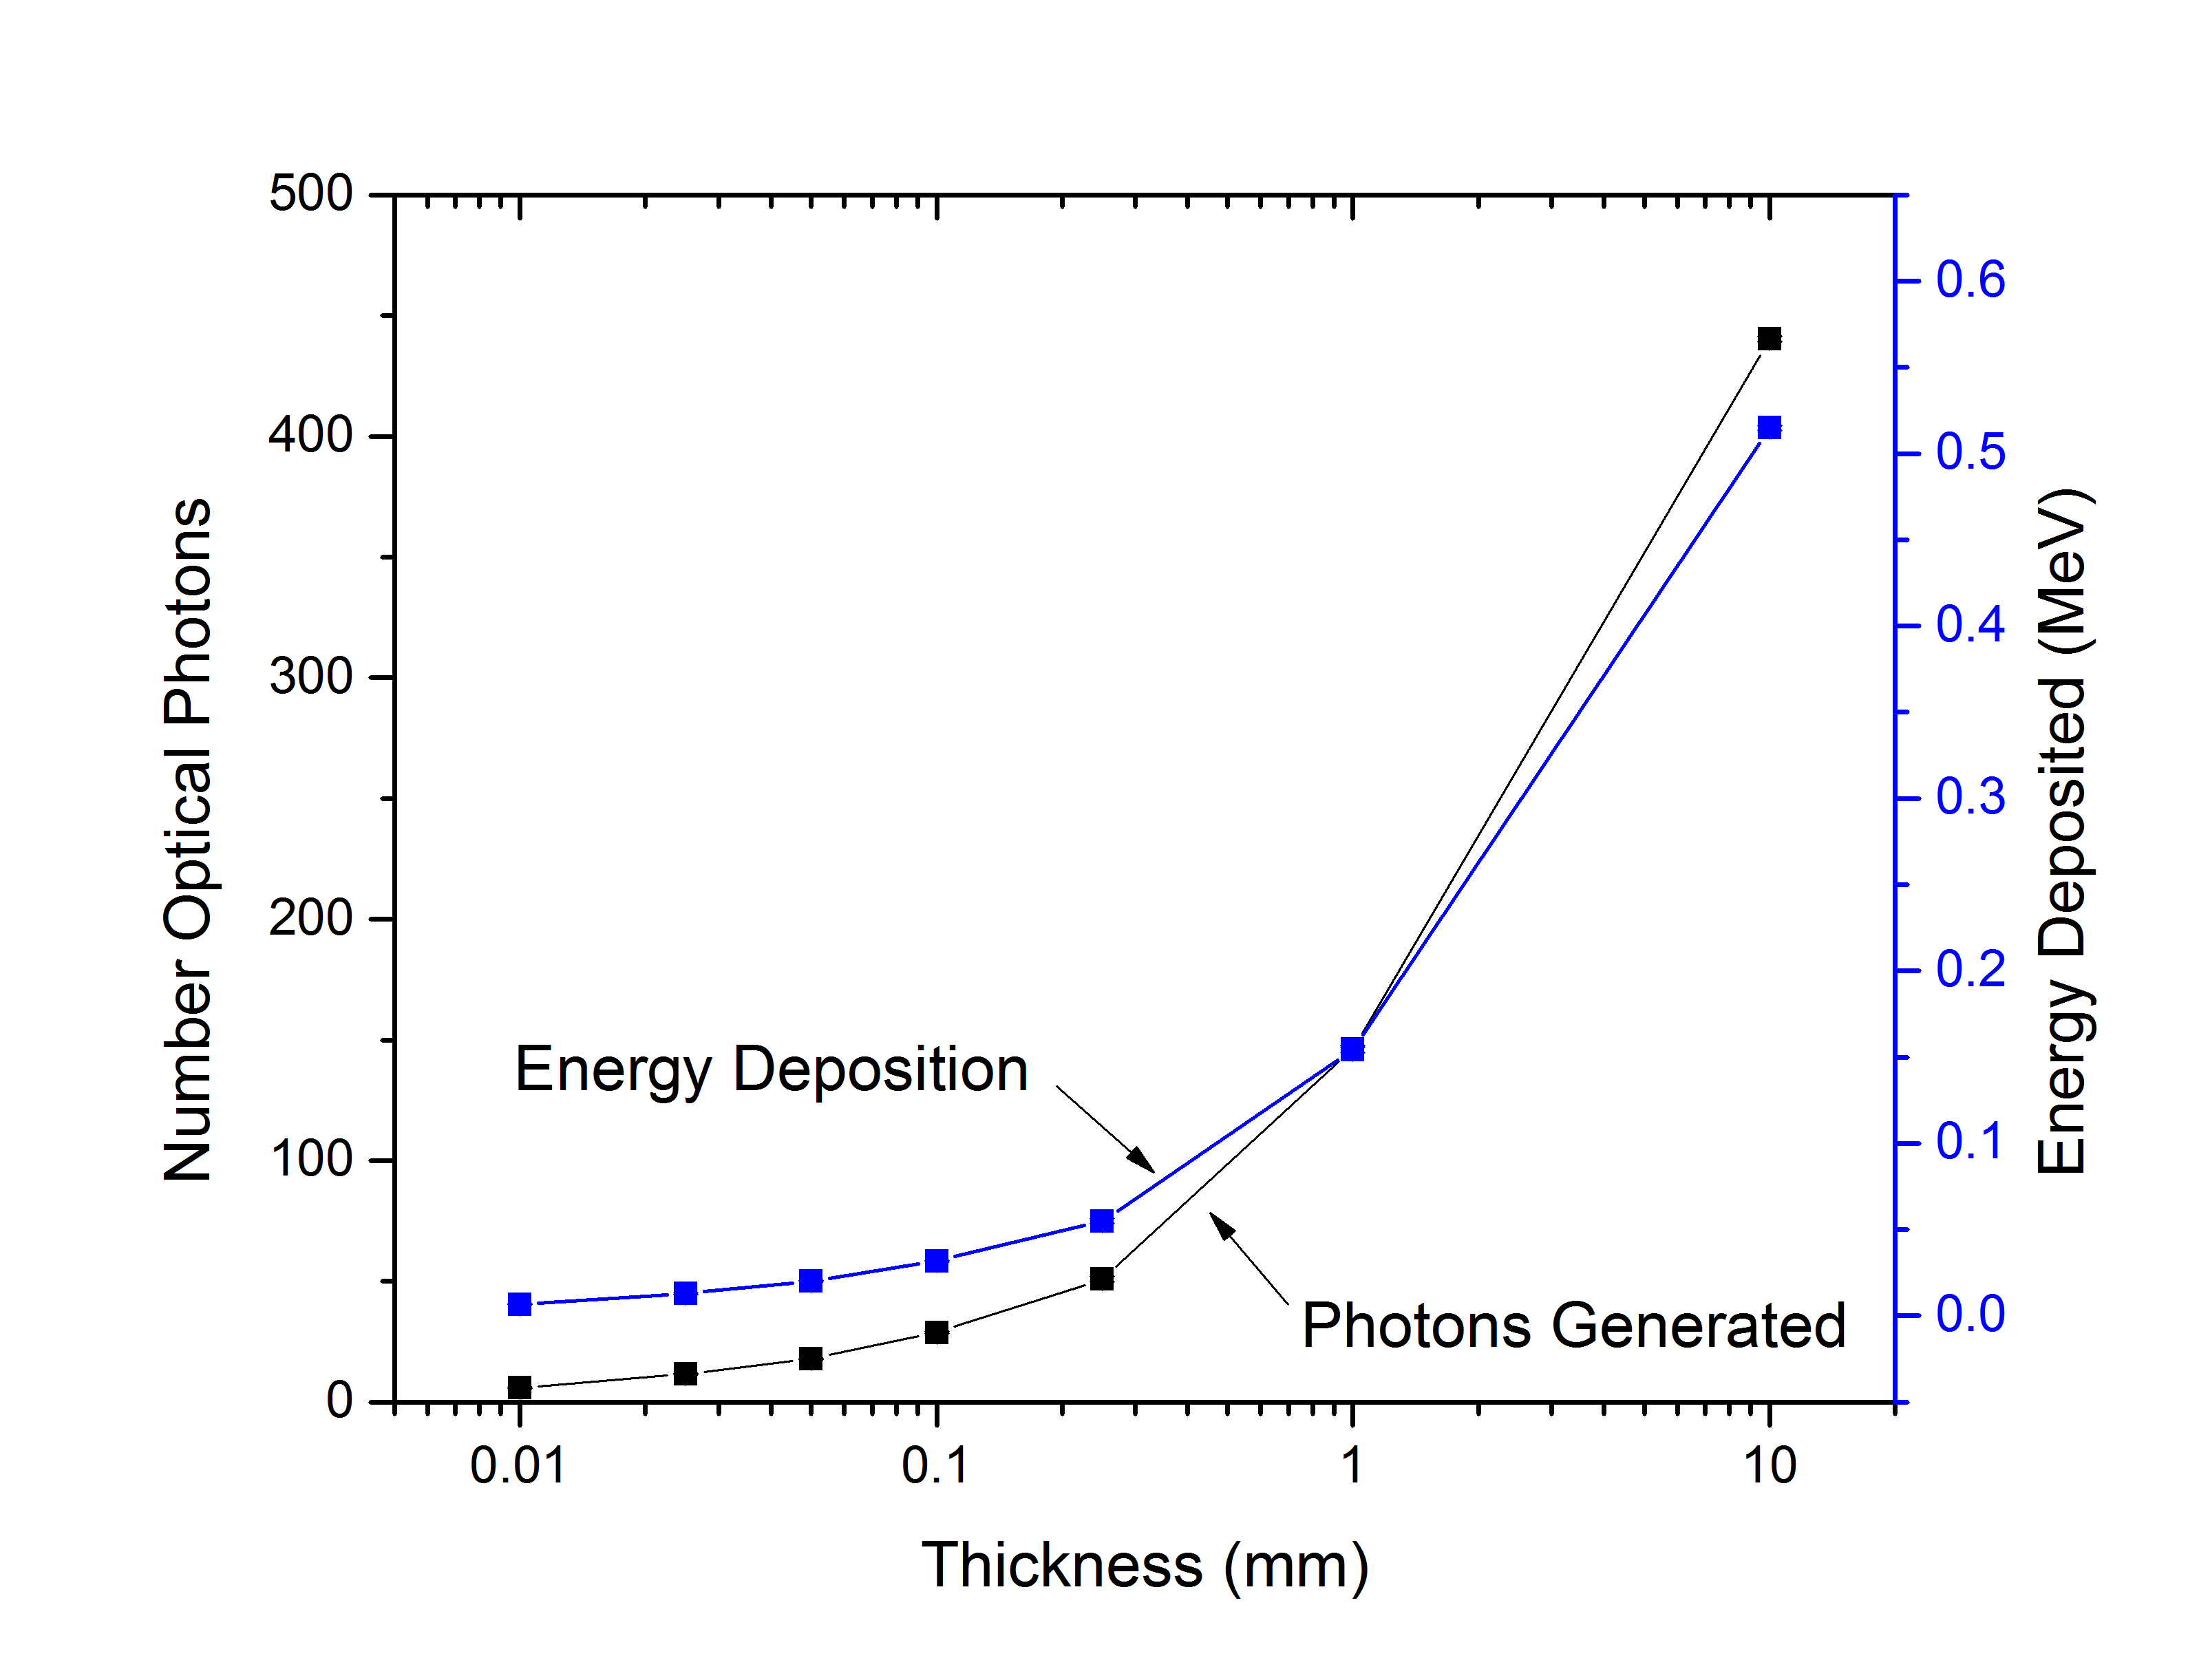
\includegraphics[width=\textwidth]{EDepLightYield_Gamma}
		\caption{ Gamma (\iso[60]{Co}}
	\end{subfigure}%
	~
	\begin{subfigure}[b]{0.45\textwidth}
    		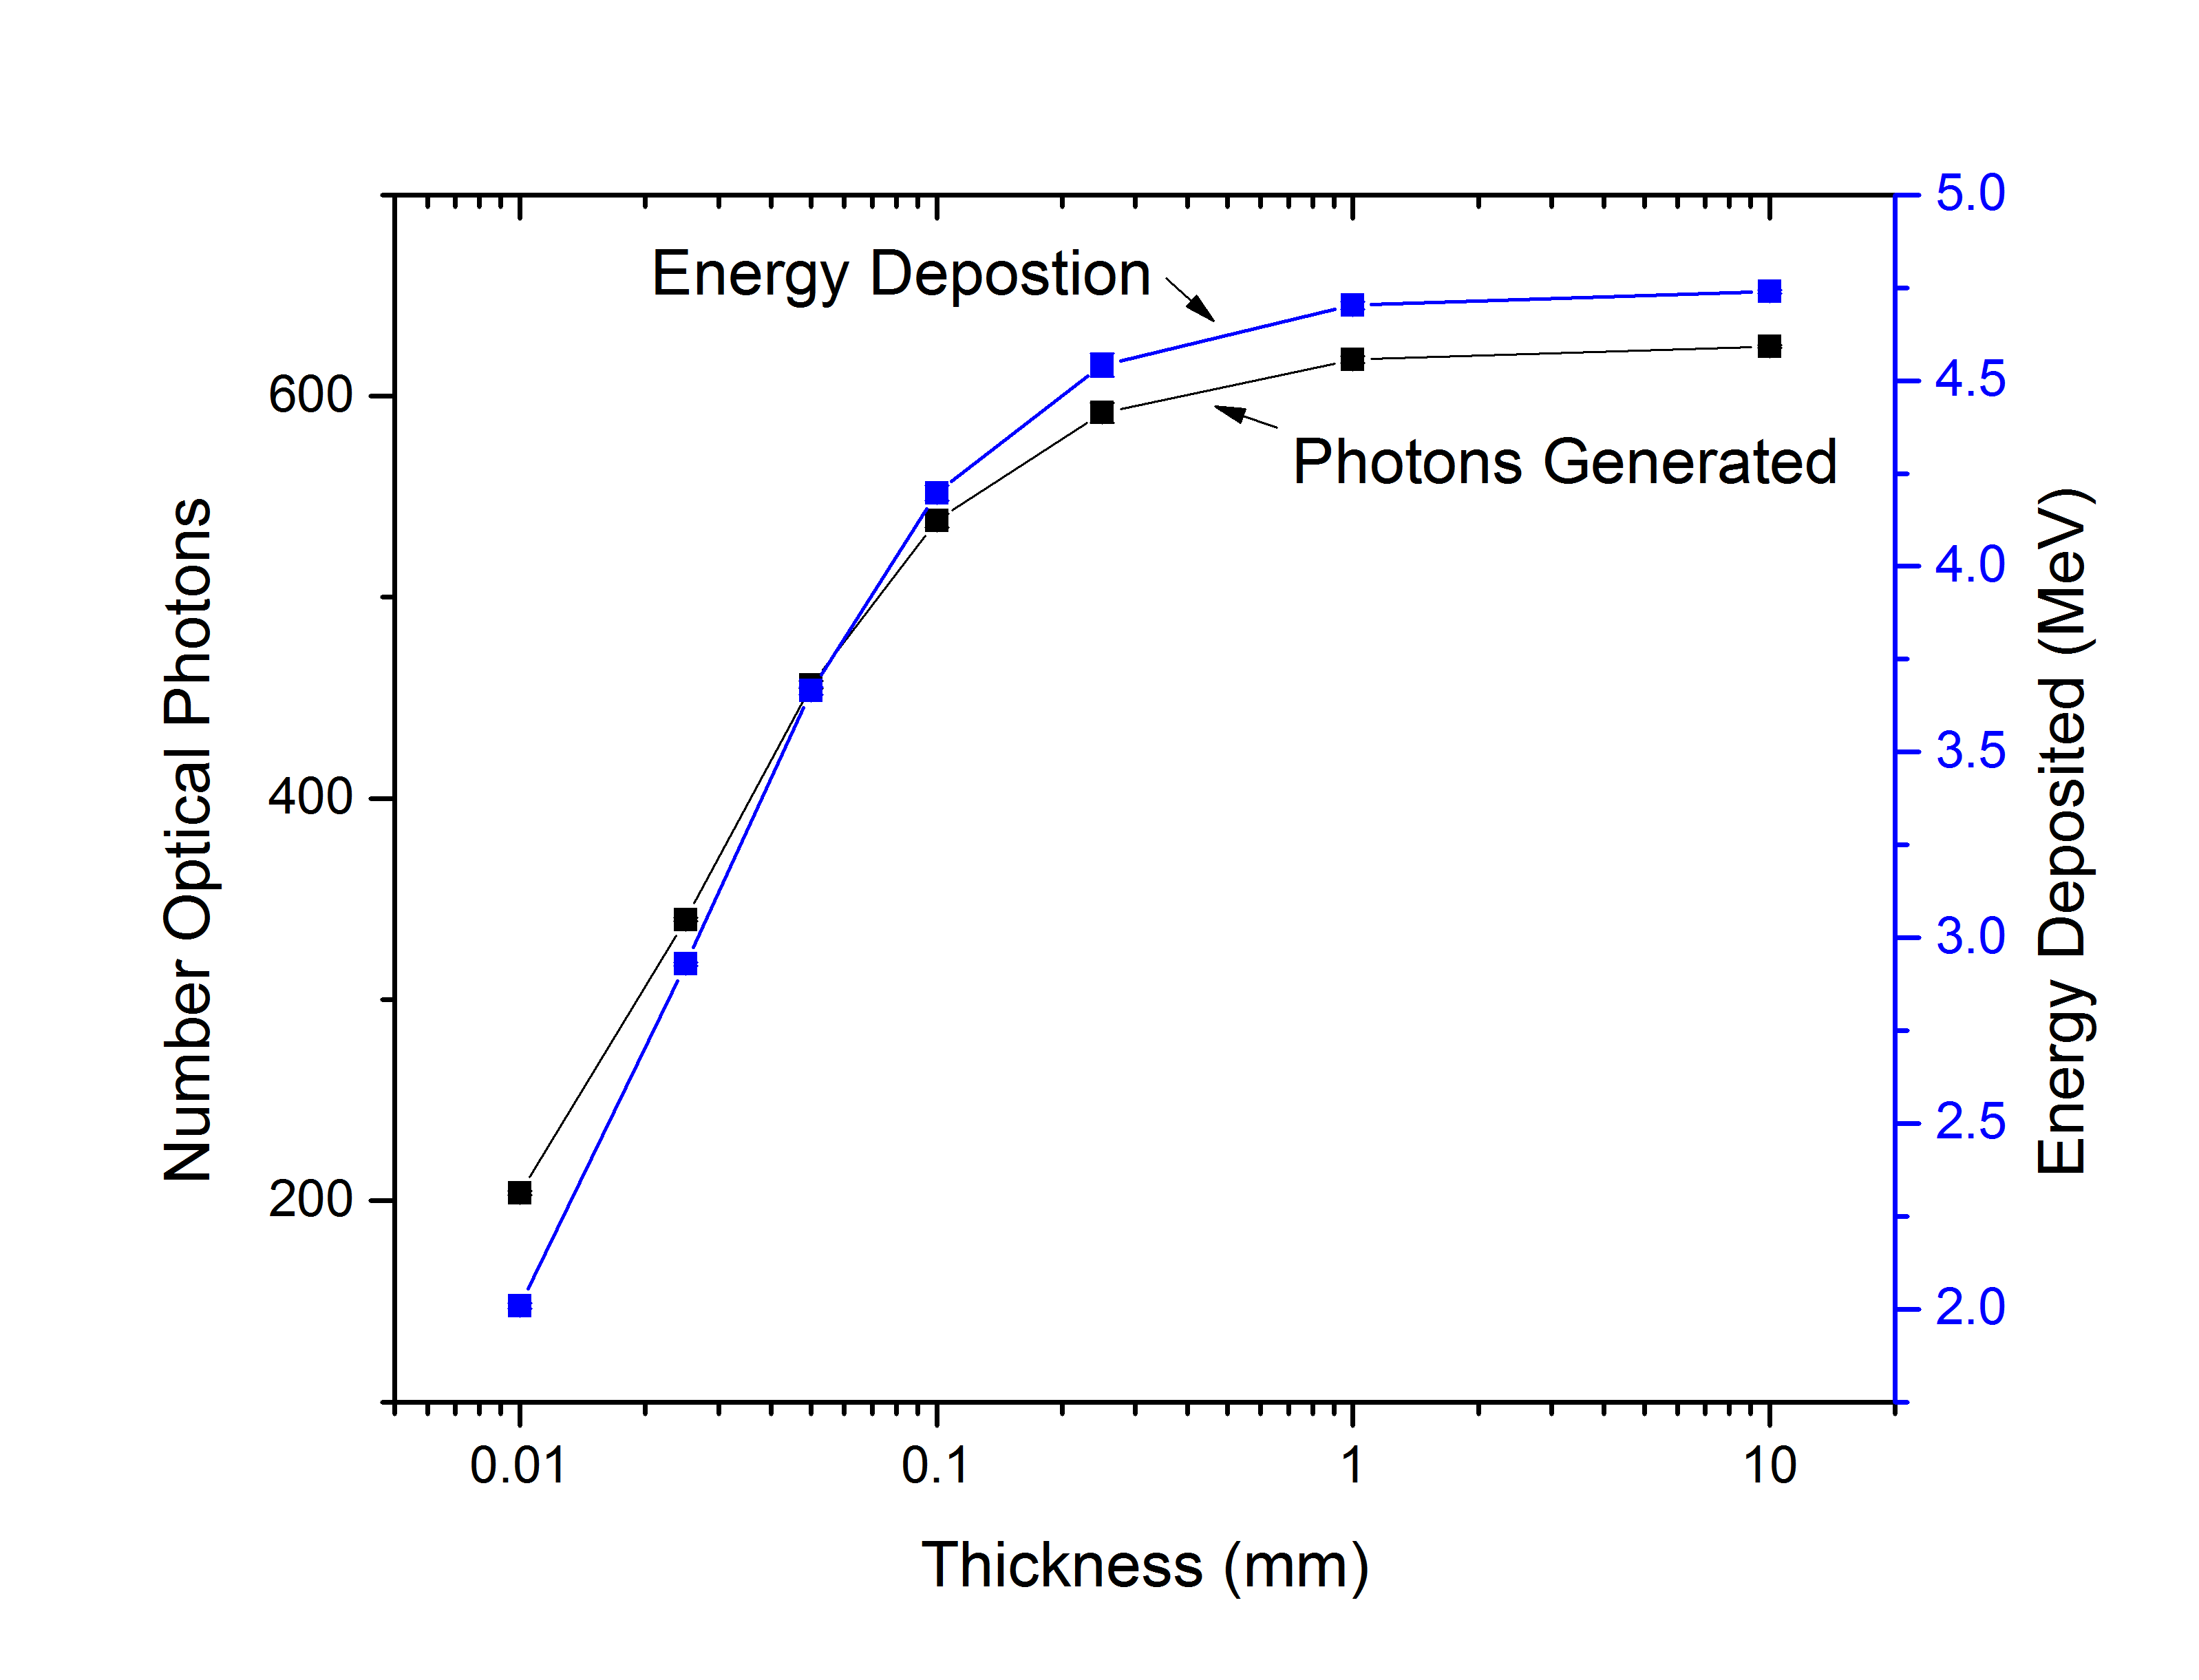
\includegraphics[width=\textwidth]{EDepLightYield_Neutron}
		  \caption{ Neutron}
	\end{subfigure}%
  \caption[Energy Deposition and Light Yield]{Simulated energy deposition and light yield.  The light yield is fairly linear with the energy deposition, thus, the energy deposition is an adequate indicator of the expected light yield.}
  \label{fig:EDepLightYield}
\end{figure*}
However, it is instructive to look at the distributions of how many photons were created per event.
As the films become thicker and more of the triton energy is captured the response of the triton starts to dominate the alpha (\autoref{fig:NeutronPhotonsGenSim}), resulting in the number of photons peaking around around 650 photons for this simulated sample.
For photons, shown in \autoref{fig:GammaPhotonsGenSim}, it is observed that the distribution is flat for very thick films, but for thinner films the probability is greatly increased for an event to generate a low number of photons.
\begin{figure}
  \centering
  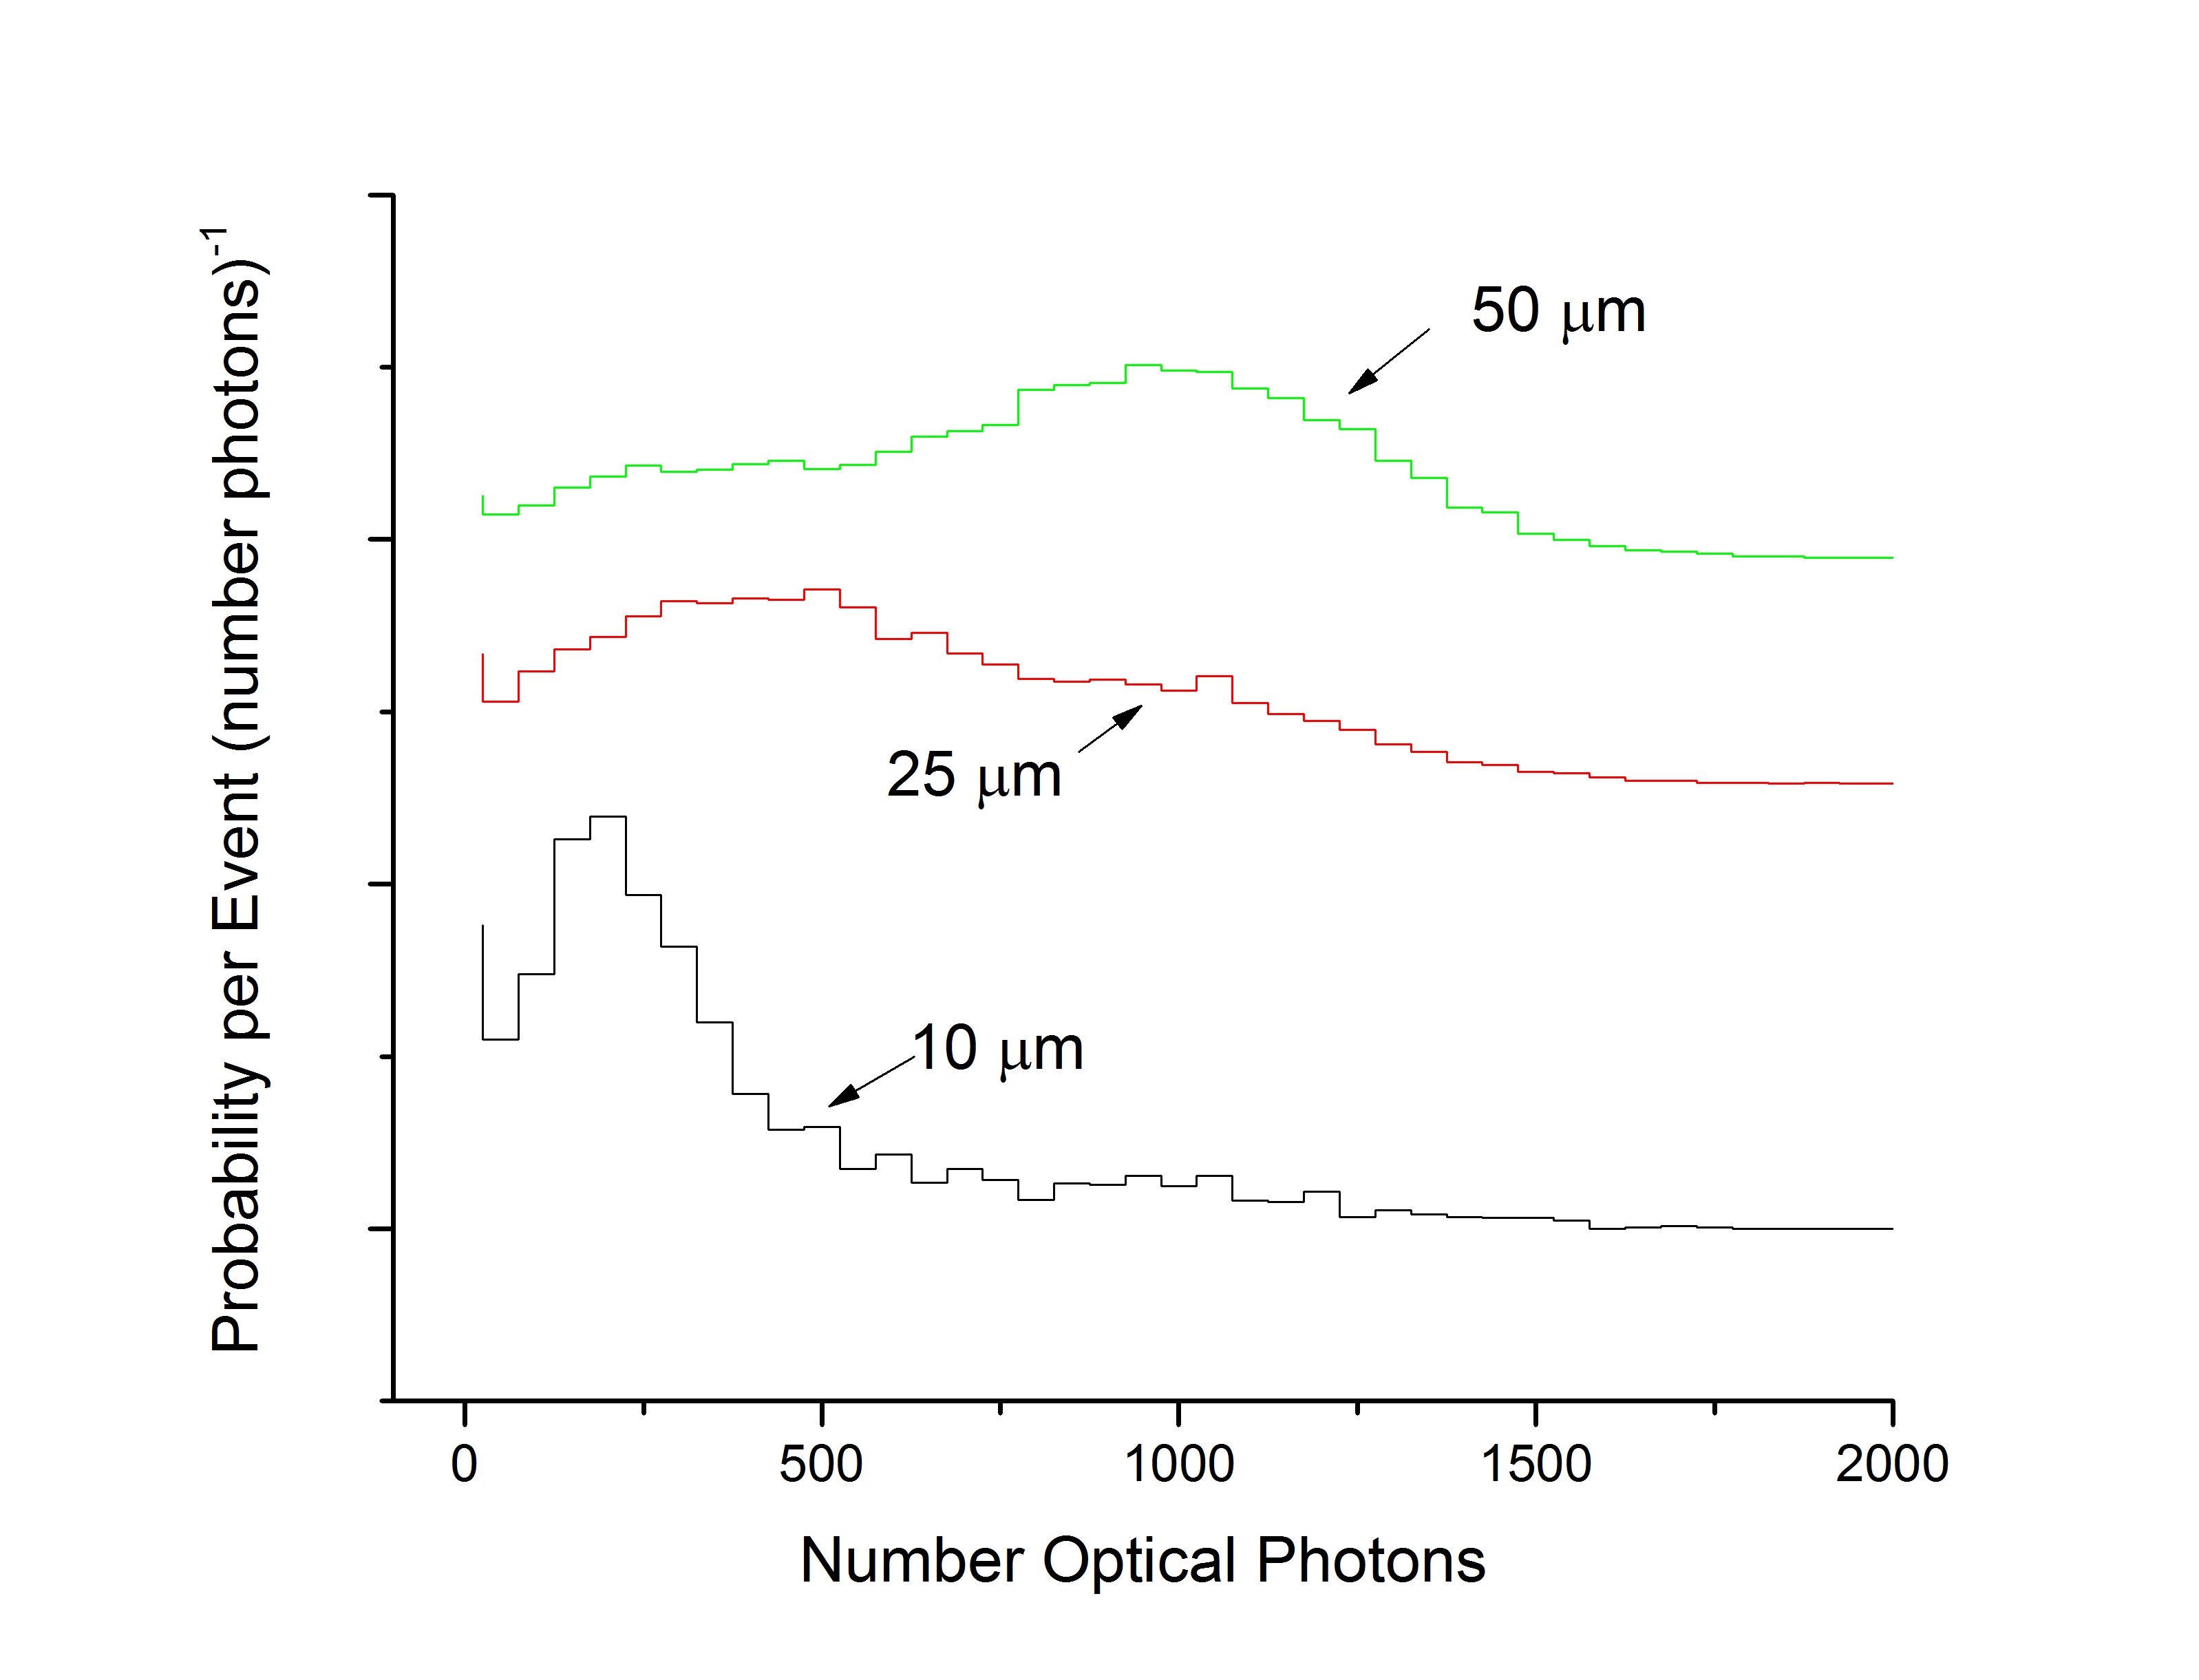
\includegraphics[width=\textwidth]{Neutron_PhotonsGenerated_Sim}
  \caption[Number of photons generated from neutron interactions]{Simulated number of photons generated from neutron interactions.  For the \SI{10}{\um} film it is observed that the majority of the photons are generated by a partial energy deposition corresponding to the alpha particle, and this effect tappers off as the films get thicker}
  \label{fig:NeutronPhotonsGenSim}
\end{figure}
\begin{figure}
  \centering
  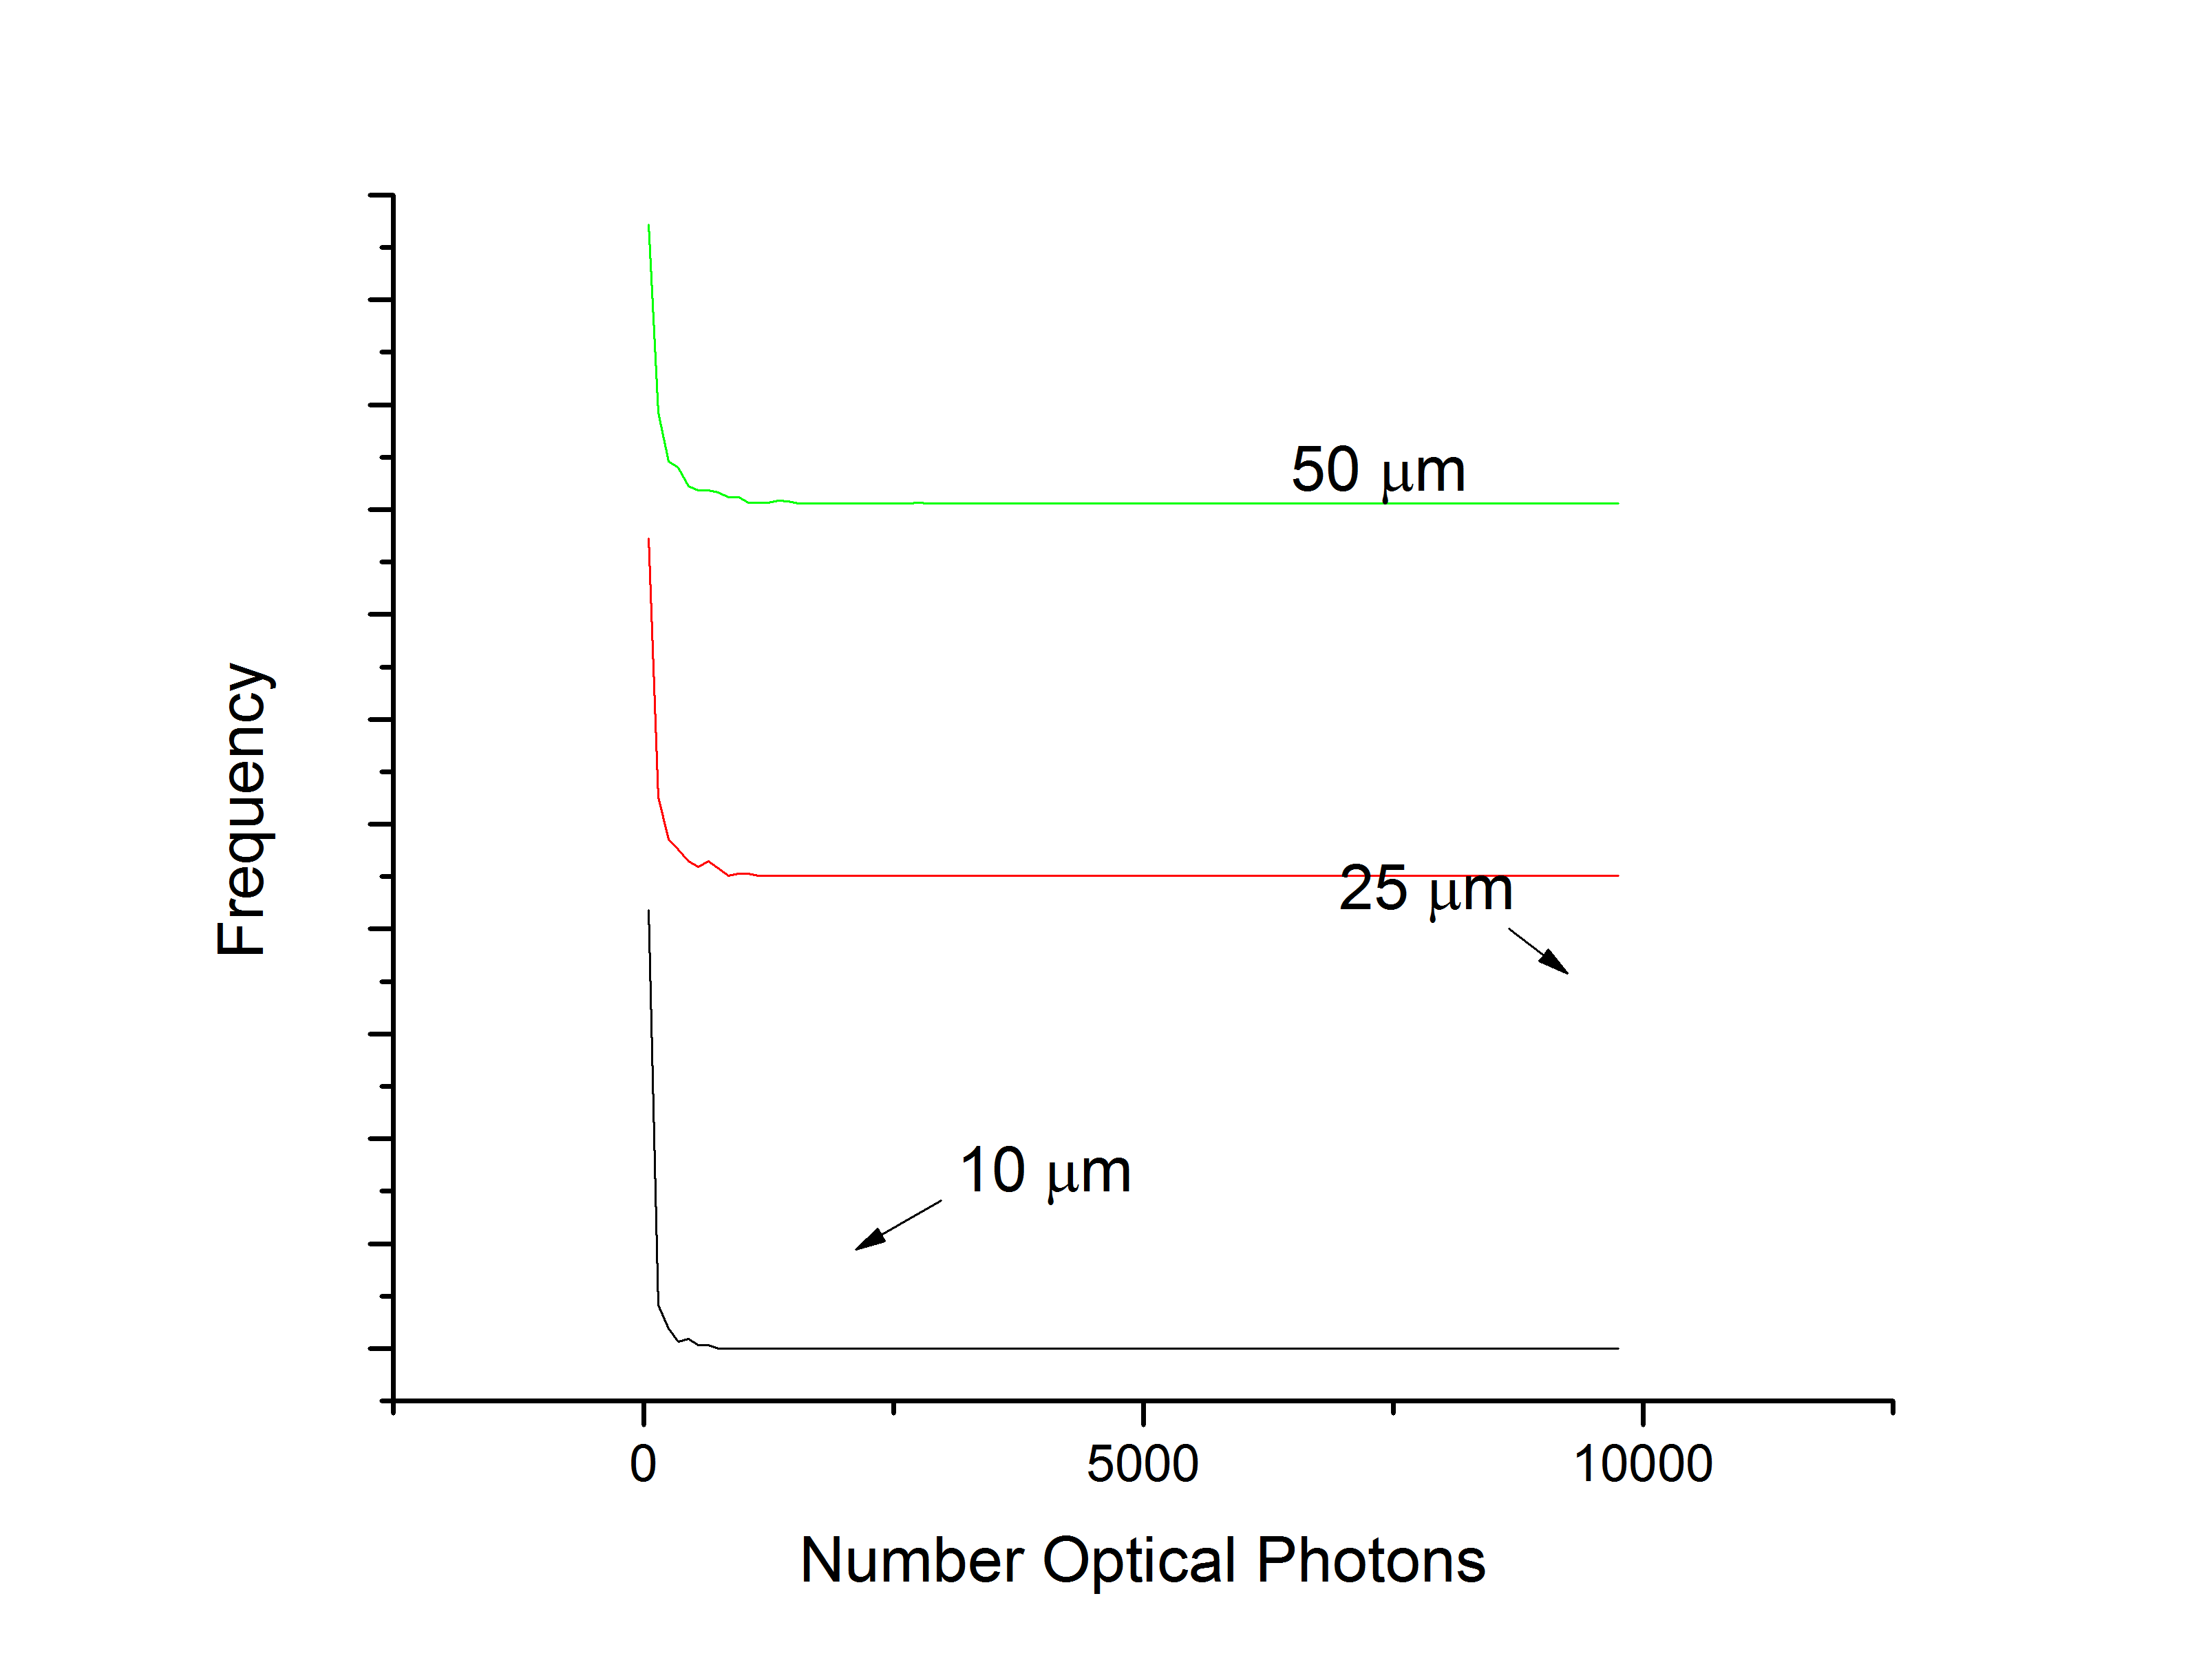
\includegraphics[width=\textwidth]{Gamma_PhotonsGenerated_Sim}
  \caption[Number of photons generated from gamma interactions]{Simulated number of photons generated from gamma interactions.}
  \label{fig:GammaPhotonsGenSim}
\end{figure}
\begin{figure}
  \centering
  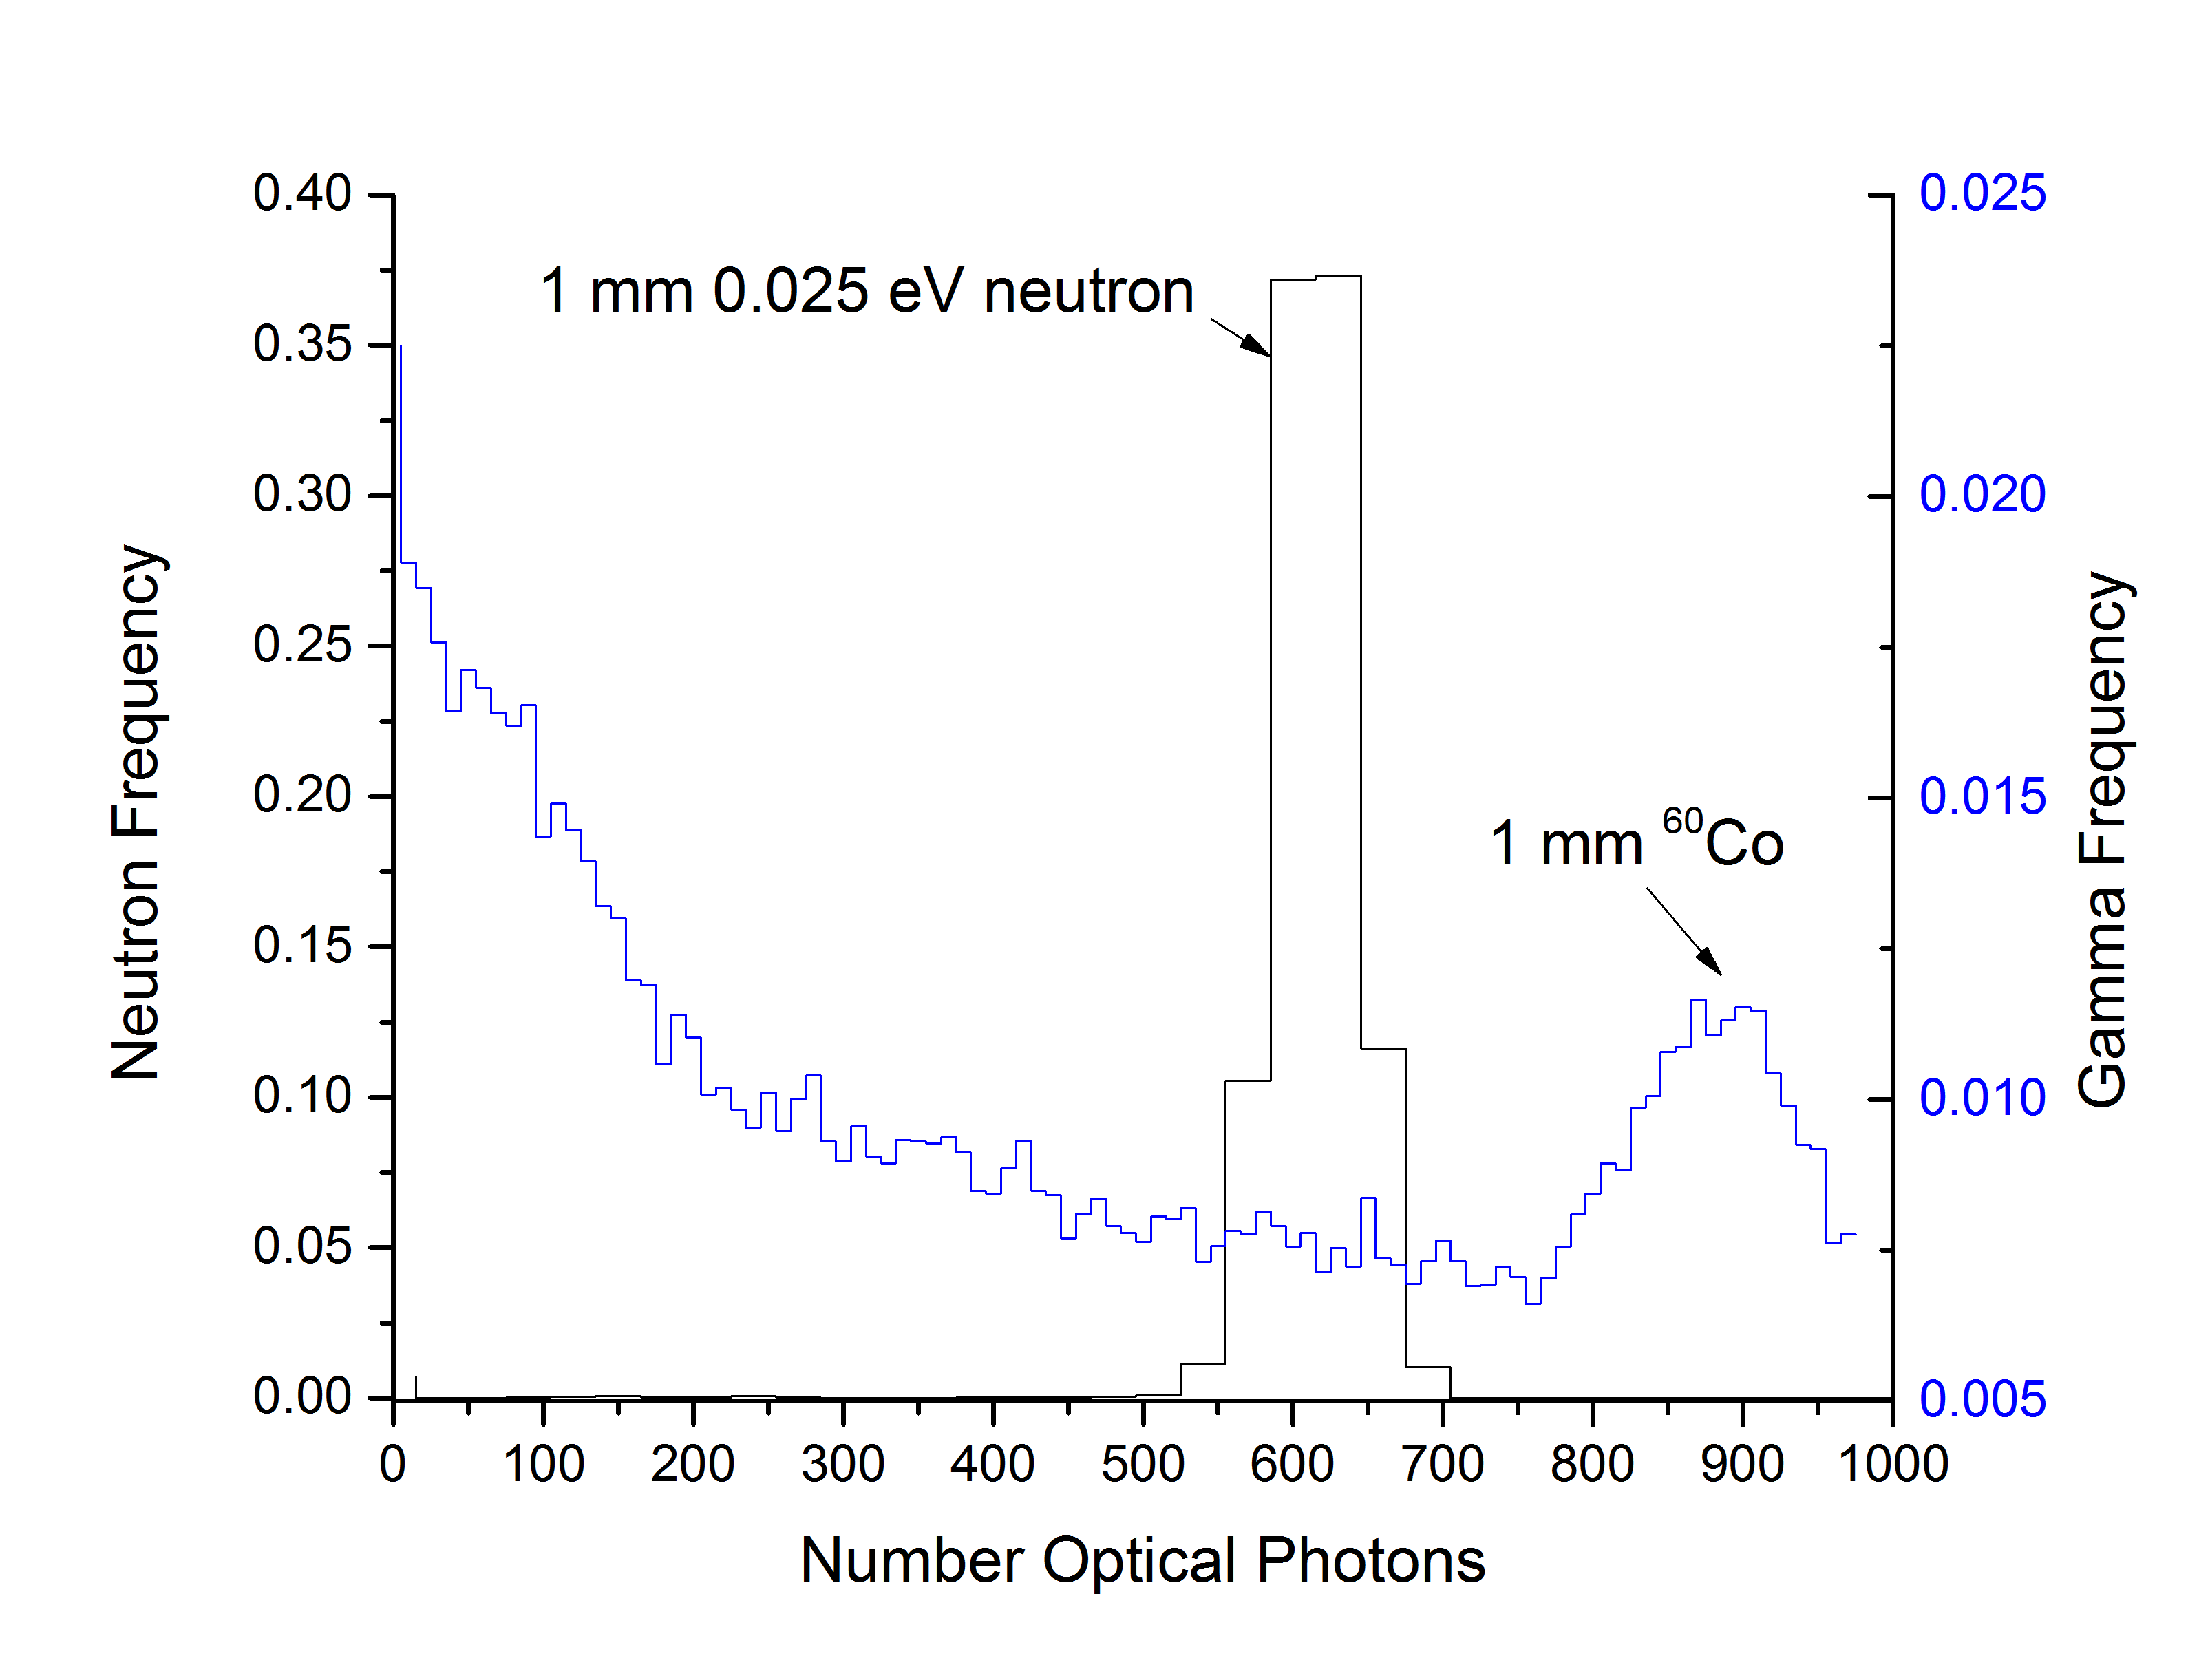
\includegraphics[width=\textwidth]{NeutronGamma_PhotonsGenerated_Sim}
  \caption[Number of photons generated of a 1 mm for neutron and gamma interactions]{Simulated number of photons generated from neutron and gamma interactions.}
  \label{fig:NeutronGammaPhotonsGenSim}
\end{figure}
